

\section{Semi-supervised Video Object Segmentation}

This task aims to segment target objects throughout a video, given only a fully-annotated mask in the first frame. Early VOS methods \cite{voigtlaender_online_2017, caelles_one-shot_2017, maninis_video_2019} employ online first-frame finetuning, which is very slow in inference, and the quality of masks gradually decreases to the end of the video. 


\begin{figure}[b!]
    \centering
    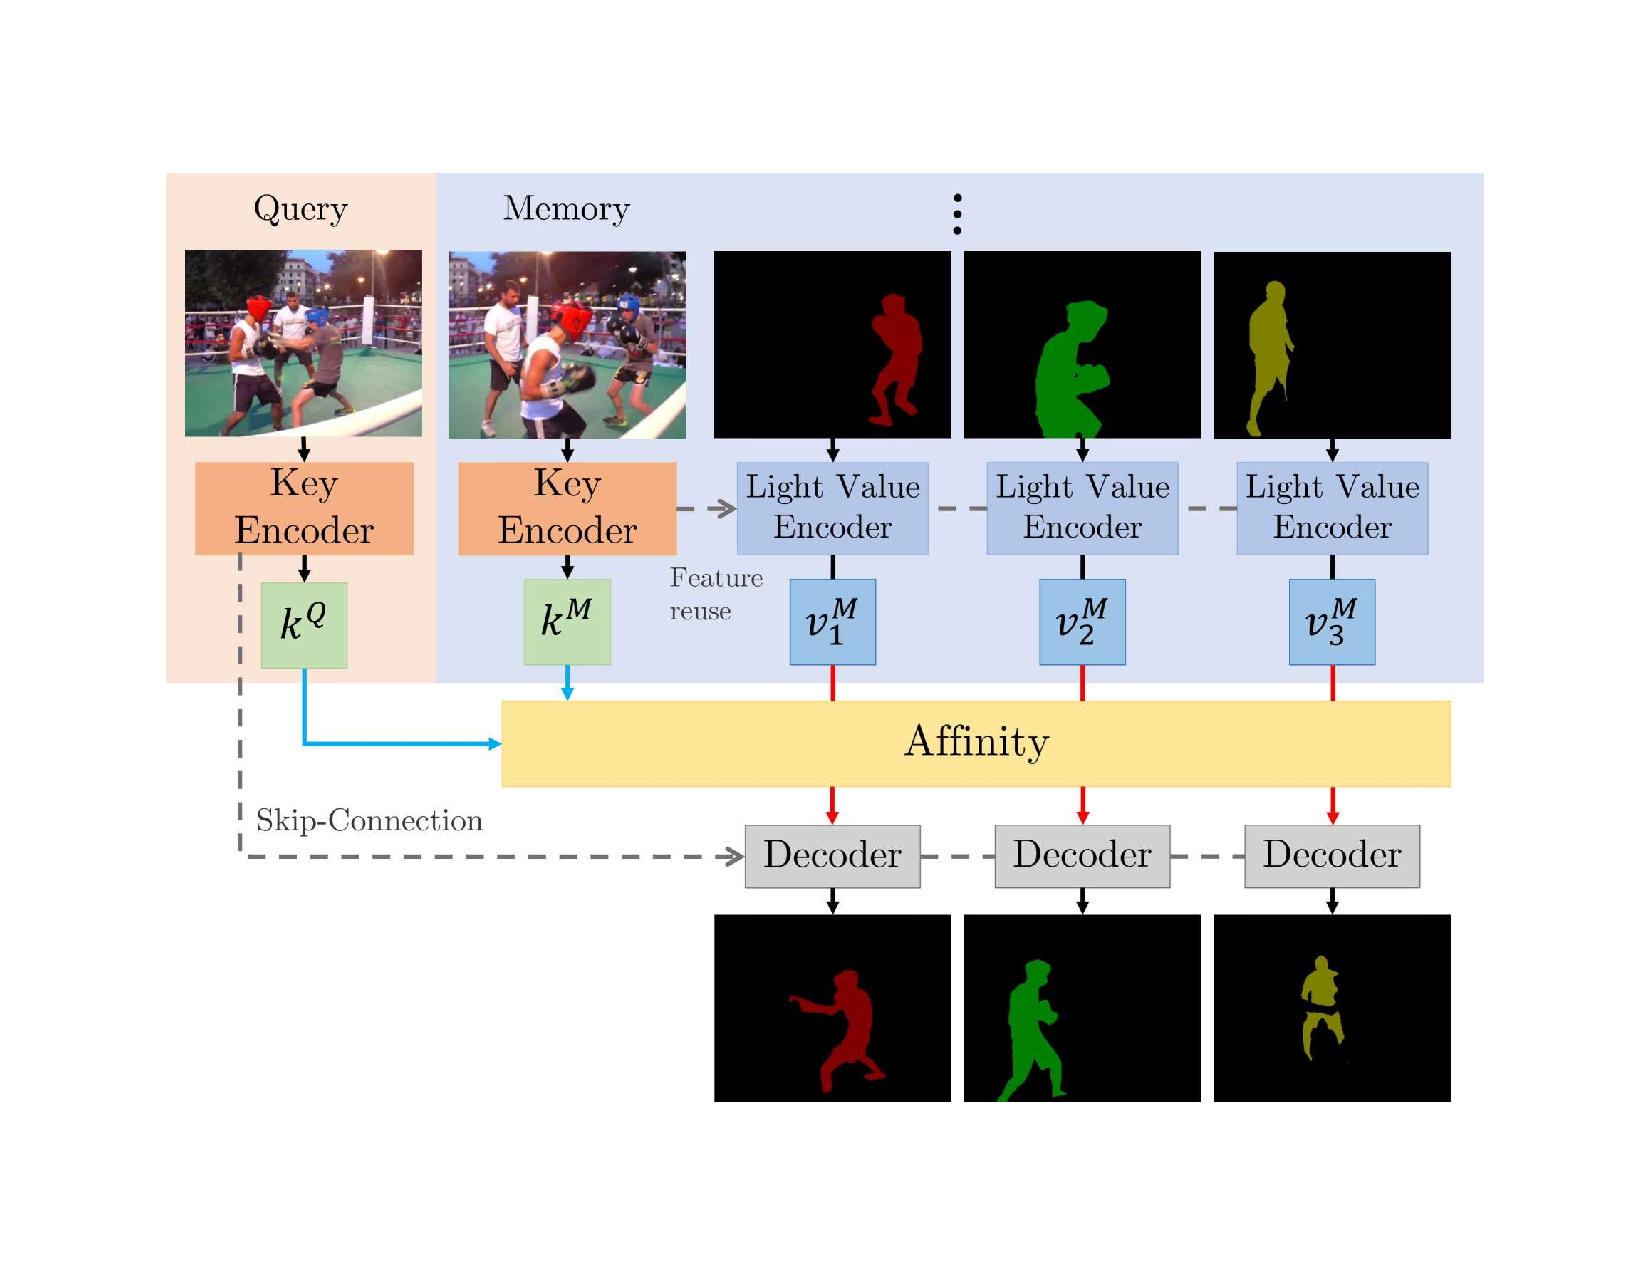
\includegraphics[width=\textwidth]{content/resources/images/STCN.pdf}
    \caption{The overview of Space-Time Correspondence Networks (STCN)\cite{cheng_rethinking_2021} }
    \label{fig:stcn}
\end{figure}

Most recent works \cite{oh_video_2019, cheng_rethinking_2021, yang_associating_2021} perform a memory feature matching. In particular, STM\cite{oh_video_2019} leverages a memory bank from past frames and utilizes the query-key-value attention mechanism to predict the mask of the current frame. AOT\cite{yang_associating_2021} constructs hierarchical matching based on a Long Short-Term Transformer.

Space-Time Correspondence Network (STCN)\cite{cheng_rethinking_2021}, inherited from STM, uses direct image-to-image correspondence for more robust matching with a modified similarity function between memory and target frame, leading to a simple, fast and efficient framework (Figure \ref{fig:stcn})

% In the scope of this thesis, we utilize the strong ability of mask propagation of STCN as a post-process to refine the high-quality mask for the entire video. 

In the scope of this project, we utilize the strong ability of mask propagation of STCN as a post-process to refine the high-quality mask for the entire video. 
